% !TeX spellcheck = en_US
\documentclass[12pt,a4paper]{article}
\usepackage[utf8]{inputenc}
\usepackage[german]{babel}
\usepackage[T1]{fontenc}
\usepackage{amsmath}
\usepackage{amsfonts}
\usepackage{amssymb}
\usepackage{graphicx}
\usepackage[left=2.5cm,right=2.5cm,top=2cm,bottom=2cm]{geometry}
\usepackage{float}

\usepackage{subcaption}
\usepackage{siunitx}
\usepackage{verbatim} 
\usepackage{flafter}
\usepackage{placeins} %\FloatBarrier

\author{Gruppe B2 \\ Máté Farkas, Maria Spethmann}
\title{Protokoll Optik 1 \\ Prismenspektrometer \\ Physikalisches Grundpraktikum 2}


\begin{document}
	\maketitle
	\thispagestyle{empty} % Keine Seitenzahl auf der Titelseite
	\newpage
	\pagestyle{headings} % Seitenzahlen oben, Section und Subsection in Kopfzeile
	\tableofcontents
	\newpage

\section{Einführung}
Ziel dieses Versuchs ist es, die Dispersionskurve $n(\lambda)$ eines Prismas unbekannten Materials zu bestimmen. Dazu wird die Ablenkung der Spektrallinien einer Quecksilber-Cadium-Lampe mithilfe eines Prismenspektrometers gemessen. Nachdem die Dispersionskurve bestimmt wurde, wird eine Spektrallinie einer Zinklampe vermessen und die berechnete Wellenlänge mit dem Literaturwert verglichen. Schließlich wird das Auflösungsvermögen des Prismas anhand der gelben Hg-Doppellinie ermittelt.

\section{Physikalische Grundlagen}
Der Brechungsindex $n$ beschreiibt die Ausbreitungsgeschwndigkeit von Licht in einem Medium. $n$ ist wellenlängenabhängig, weil die Anregung der Elektronen in einem Medium durch das Verhältnis zwischen Eigenfrequenz der Elektronen und Frequenz der elektromagnetischen Welle bestimmt wird. Im Bereich des sichtbaren Lichtes lässt sich die Dispersionskurve $n(\lambda)$ durch die Cauchy-Gleichung annähern
\begin{equation}\label{eq:Cauchy-Gleichung}
n(\lambda)=a+\frac{b}{\lambda^2}+\frac{c}{\lambda^4},
\end{equation}
wobei $a$, $b$ und $c$ materialabhängige Konstanten sind.\\
Wenn Licht auf Materie trifft, wird der Lichtstrahl gebrochen. Das Snelliussche Brechungsgesetz bezieht Einfallswinkel $\alpha_1$, Brechungswinkel $\alpha_2$ und die Brechungsindexe der Medien aufeinander:
\begin{equation}
n_1 \cdot sin(\alpha_1) = n_2 \cdot sin(\alpha_2)
\end{equation}
Mithilfe dieses Gesetzes und geometrischen Zusammenhängen kann der Strahlengang durch ein Prisma berechnet werden.
\begin{figure}[H]
	\centering
	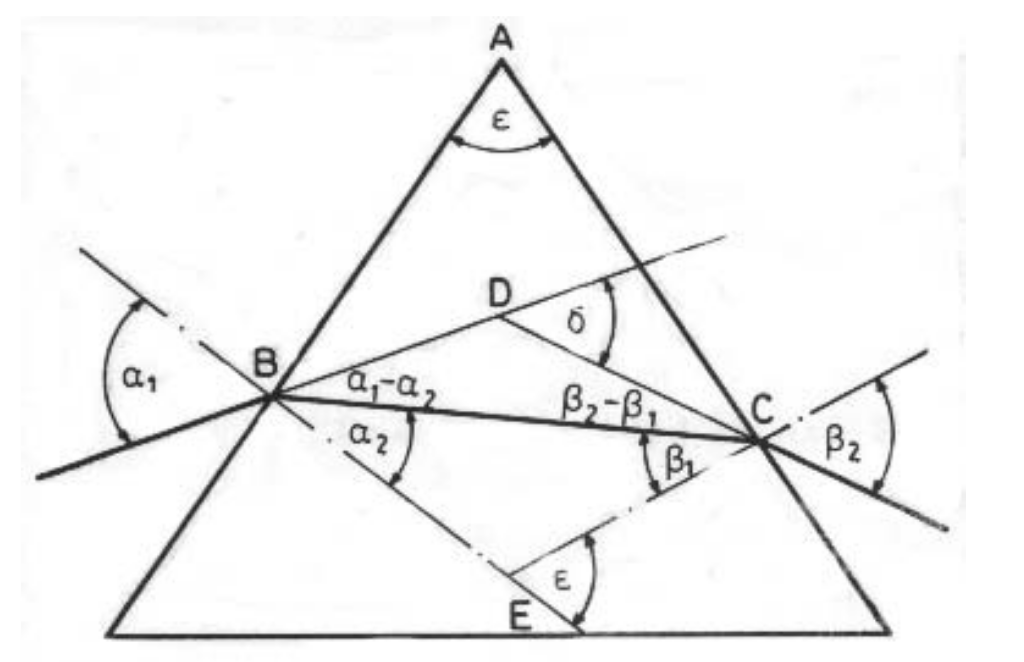
\includegraphics[width=0.8\textwidth]{Prisma_Strahlengang.png}
	\caption{Strahlengang durch das Prisma (Quelle: Praktikumsskript)}
	\label{Prisma_Strahlengang}
\end{figure}
Der Ablenkwinkel $\delta$ wird minimal für den symmetrischen Strahlendurchgang, bei dem der Austrittwinkel $\beta_2$ gleich dem Einfallswinkel $\alpha_1$ ist. In diesem Fall gilt folgender Zusammenhang zwischen Minimalablenkung und Brechungsindex:
\begin{equation}\label{eq:n_aus_delmin}
n=\frac{\sin((\delta_{min}+\epsilon)/2)}{\sin(\epsilon/2)}
\end{equation}
In diesem Versuch wird die Minimalablenkung $\delta_{min}$ bekannter Spektrallinien des Cadmiums- und Quecksilberspektrums gemessen und daraus der Brechungsindex berechnet. Nun können die Koeffizienten $a$, $b$ und $c$ der Cauchy-Gleichung (Gl.~\eqref{eq:Cauchy-Gleichung}) mit einer Ausgleichsrechnung bestimmt werden.\\\\
Eine charakterisierende Größe eines Prismas ist sein Auflösungsvermögen $A$. Es wird definiert als 
\begin{equation}
A=\frac{\lambda}{\Delta\lambda}
\end{equation}
und beschreibt die benötigte Wellenlängendifferenz $\Delta\lambda$, um zwei Spektrallinien mit Wellenlängen $\lambda$ und $\lambda+\Delta\lambda$ noch mit dem Prisma trennen zu können. Bei symmetrischem Strahlengang und voller Ausleuchtung lässt sich das Auflösungsvermögen des Prismas berechnen durch
\begin{equation}
A=S\frac{dn}{d\lambda}
\end{equation}
mit Prismenbasis $S$.
\section{Allgemeiner Versuchsaufbau und Durchführung}
Der Versuchsaufbau besteht aus einer Lichtquelle, einem festen Kollimator, einem Prisma auf einer Drehscheibe und einem schwenkbaren Fernrohr, dessen Winkeleinstellung bezüglich eines festen Teilkreises auf eine Bogenminute genau abgelesen werden kann. Das Licht der Spektrallampe fällt über einen Spalt, dessen Breite die Intensit"at regelt, in den Kollimator und wird an der Kollimatorlinse in ein ebenes Lichtbündel umgewandelt. Das Lichtbündel fällt auf das Prisma und wird abhängig von Einfallswinkel und Wellenlänge abgelenkt. Nun kann das abgelenkte Bild des Spaltes durch das Fernrohr vergrößert betrachtet werden, das aus einer Objektiv- und einer Okularlinse besteht. Der Strahlengang durch das Spektrometer wird in Abb.~\ref{Spektrometer_Aufbau} dargestellt. Abb.~\ref{Aufbau_Foto} zeigt eine Übersicht über den Versuchsaufbau (einschließlich der für Teilversuch 3 benötigten Schlitzblende).\\
Bei Teilversuch 1 und 2 wird für jede Messung die Minimalablenkung eingestellt. Dazu betrachtet man durch das Fernrohr eine Spektrallinie und variiert durch Drehung der Prismadrehscheibe den Einfallswinkel. Ein symmetrischer Strahlendurchgang mit Minimalablenkung ist dann erreicht, wenn sich bei gleichsinniger Drehung des Prismas die Laufrichtung des Spaltbildes durch das Fernrohr umkehrt. Man schwenkt den Fernrohrarm so, dass sich das Fadenkreuz des Fernrohrs dann auf dem Spalt befindet, wenn die Minimalablenkung erreicht ist, und notiert den Winkel der Fernrohrposition $\psi_1$. Anschließend dreht man das Prisma um, sodass das Licht auf die andere Seite gebrochen wird, wiederholt den beschriebenen Prozess zum Finden des symmetrischen Strahldurchgangs und misst den zweiten Winkel $\psi_2$, der zur gleichen Spetkrallinie gehört. Die Minimalauslenkung $\delta_{min}$ lässt sich nun berechnen durch
\begin{equation}\label{eq:delmin_aus_psi}
\delta_{min}=\frac{\psi_1-\psi_2}{2}.
\end{equation}

\begin{figure}[H]
	\centering
	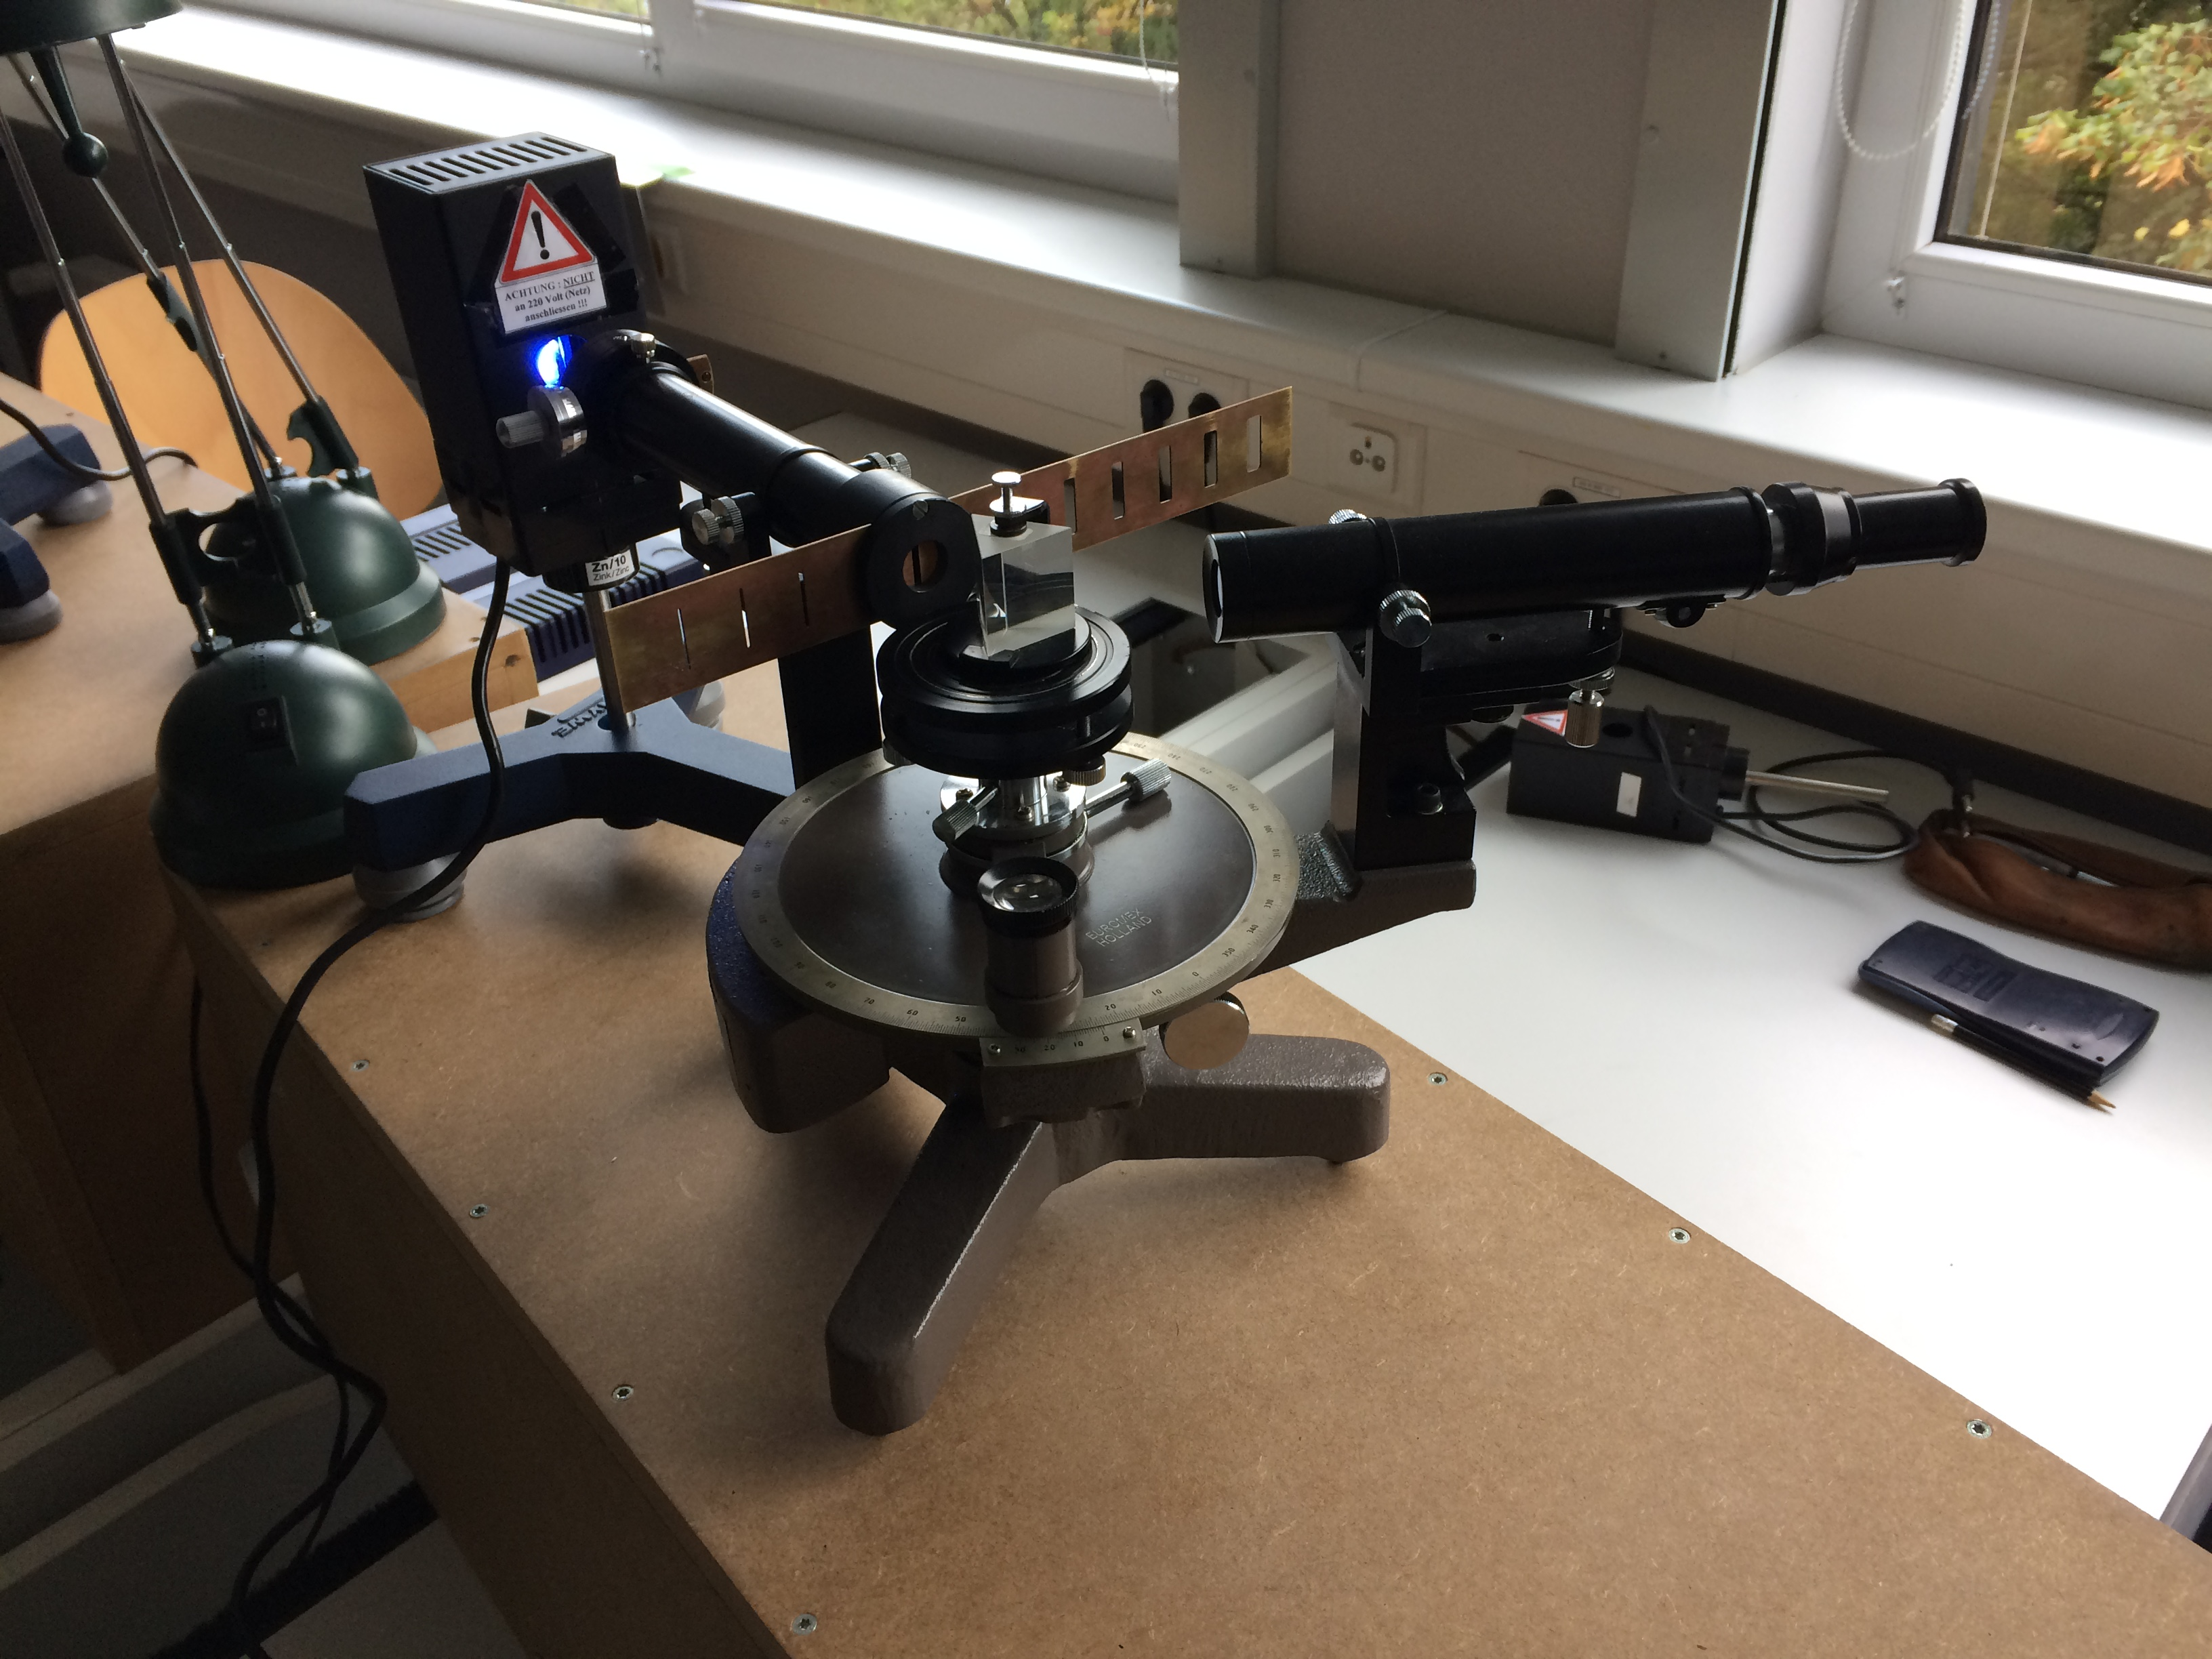
\includegraphics[width=0.9\textwidth]{Aufbau_Foto.jpg}
	\caption{Versuchsaufbau}
	\label{Aufbau_Foto}
\end{figure}
\begin{figure}[H]
	\centering
	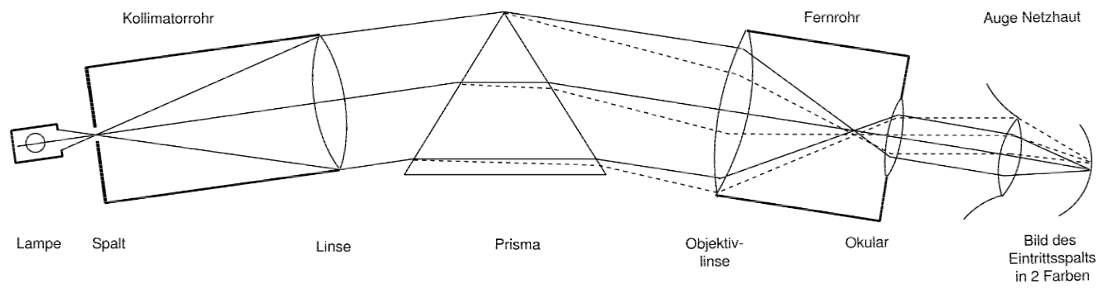
\includegraphics[width=0.9\textwidth]{Spektrometer_Aufbau.png}
	\caption{Versuchsaufbau: Strahlengang durch das Spektrometer (Quelle: Praktikumsskript)}
	\label{Spektrometer_Aufbau}
\end{figure}

\section{Bestimmung der Dispersionskurve $n(\lambda)$}

\subsection{Versuchsdurchführung}

Zunächst verwenden wir eine Hg/Cd-Lampe und messen für sechs ausgewählte Spektrallinien  jeweils drei Mal die linksseitigen und rechtsseitigen Umkehrwinkel $\psi_1$ und $\psi_2$ (siehe Tabelle \ref{table:Winkel_Rohdaten}). Die Werte werden gemittelt und der Brechungsindex in Abhängigkeit der Wellenlängen mithilfe von Gl.~\eqref{eq:delmin_aus_psi} und Gl.~\eqref{eq:n_aus_delmin} berechnet. Um den Fehler der Messgenauigkeit abschätzen zu können, wird $\psi_1$ der roten Spektrallinie von Quecksilber 10 Mal bestimmt. Die Unsicherheit auf dieses $\psi_1$ wird auf die anderen Messungen übertragen, da angenommen wird, dass sie der gleichen statistischen Verteilung folgt.

\subsection{Bestimmung der Messunsicherheit auf  $\psi_i$}
Die gemessenen Werte für $\psi_{1}$ und $\psi_2$ sind in Tabelle \ref{table:Winkel_Rohdaten} zusammengefasst. Zur Bestimmung der Messunsicherheit auf $\psi$ verwenden wir die 10 linksseitigen Messungen $\psi_1$ der roten Cadmiumlinie. Abb.~\ref{Histogramm} zeigt ein Histogramm dieser 10 Messungen. Es ist zu erkennen, dass die Streuung recht gro\ss  ist, deutlich gr"o\ss er als die Winkelskala des Fernrohrs.
\begin{figure}[H]
	\centering
	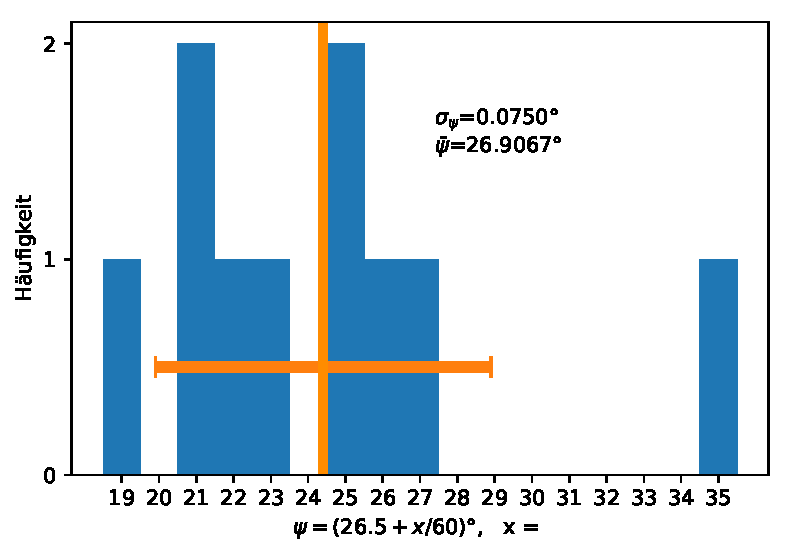
\includegraphics[width=0.6\linewidth]{Python/Histogramm_Psi.pdf}
	\caption{Histogramm der 10 linksseitigen Messungen der roten Cadmiumlinie. Orange markiert sind Mittelwert und Standardabweichung}
	\label{Histogramm}
\end{figure}
Wir berechnen die Standardabweichung der Verteilung durch
\begin{equation}
\sigma_{\psi}=\sqrt{\frac{1}{N-1}\sum^{N}_{i=1}{(\psi-\overline{\psi})^2}}
\end{equation}
mit $N=10$ und nehmen an, dass diese Unsicherheit auch für die anderen Werte von $\psi_1$ und $\psi_2$ gilt. Die Berechnung ergibt
\begin{equation}
\sigma_{\psi}=\ang{0.075}.
\end{equation}
Die Unsicherheit auf den Mittelwert einer Größe erhält man nun durch
\begin{equation}
\sigma_{\overline{\psi}}=\frac{\sigma_{\psi}}{\sqrt{N}}
\end{equation}
bei N Messungen.  In unserem Fall ergibt sich für drei Messungen $\sigma_{\overline{\psi}}=\ang{0.043}$, bzw. f"ur die 10 Messungen der roten Cadmiumlinie $\sigma_{\overline{\psi}}=\ang{0.024}$
\begin{table}[H]
	\centering
	\begin{tabular}{|c|c|c|}
		\hline
		& Winkel $\psi_{1i}$ in Grad & Winkel $\psi_{2i}$ in Grad\\
		\hline
		Cadmium&$26.5+\frac{27}{60}$&$144.5+\frac{21}{60}$\\[0.1cm]
		rot&$26.5+\frac{26}{60}$&$144.5+\frac{20}{60}$\\[0.1cm]
		$\lambda=643.85nm$&$26.5+\frac{25}{60}$&$144.5+\frac{20}{60}$\\[0.1cm]
		&$26.5+\frac{35}{60}$&\\[0.1cm]
		&$26.5+\frac{23}{60}$&\\[0.1cm]
		&$26.5+\frac{21}{60}$&\\[0.1cm]
		&$26.5+\frac{19}{60}$&\\[0.1cm]
		&$26.5+\frac{22}{60}$&\\[0.1cm]
		&$26.5+\frac{25}{60}$&\\[0.1cm]
		&$26.5+\frac{21}{60}$&\\[0.1cm]
		\hline
		Quecksilber&$25.5+\frac{5}{60}$&$146+\frac{15}{60}$\\[0.1cm]
		grün&$25.5+\frac{5}{60}$&$146+\frac{15}{60}$\\[0.1cm]
		$\lambda=546.07nm$&$25.5+\frac{3}{60}$&$146+\frac{16}{60}$\\[0.1cm]
		\hline
		Cadmium&$24.5+\frac{12}{60}$&$147+\frac{5}{60}$\\[0.1cm]
		blaugrün&$24.5+\frac{13}{60}$&$147+\frac{4}{60}$\\[0.1cm]
		$\lambda=508.58nm$&$24.5+\frac{14}{60}$&$147+\frac{5}{60}$\\[0.1cm]
		\hline
		Cadmium&$24.5+\frac{16}{60}$&$147.5+\frac{23}{60}$\\[0.1cm]
		hellblau&$24.5+\frac{15}{60}$&$147.5+\frac{21}{60}$\\[0.1cm]
		$\lambda=479.99nm$&$24.5+\frac{15}{60}$&$147.5+\frac{22}{60}$\\[0.1cm]
		\hline
		Quecksilber&$22+\frac{16}{60}$&$149.5+\frac{3}{60}$\\[0.1cm]
		violett&$22+\frac{17}{60}$&$149.5+\frac{2}{60}$\\[0.1cm]
		$\lambda=435.83nm$&$22+\frac{13}{60}$&$149.5+\frac{1}{60}$\\[0.1cm]
		\hline
		Quecksilber&$20.5+\frac{5}{60}$&$151+\frac{13}{60}$\\[0.1cm]
		dunkelviolett&$20.5+\frac{6}{60}$&$151+\frac{14}{60}$\\[0.1cm]
		$\lambda=404.66nm$&$20.5+\frac{6}{60}$&$151+\frac{14}{60}$\\[0.1cm]
		\hline
	\end{tabular}
	\caption{Winkel der Spektrallinien}
	\label{table:Winkel_Rohdaten}
\end{table}

\subsection{Auswertung}
Nun berechnen wir aus den gemittelten linksseitigen und rechtsseitigen Umkehrwinkeln die Minimalablenkung $\delta_{min}$ und den Brechungsindex $n$ gemäß Gl.~\eqref{eq:delmin_aus_psi} und Gl.~\eqref{eq:n_aus_delmin}. Die Unsicherheiten auf $\delta_{min}$ und $n$ werden durch Fehlerfortpflanzung ermittelt und sind statistischer Natur.
\begin{align}
\sigma_{\delta_{min}}&=\frac{1}{2}\sqrt{\sigma_{\overline{\psi_1}}^2+\sigma_{\overline{\psi_2}}^2}\\
\sigma_n&=\Big|\frac{1}{2\sin{\frac{\epsilon}{2}}}\cos{\left(\frac{\epsilon+\delta_{min}}{2}\right)}\sigma_{\delta_{min}}\Big|
\end{align}
Die systematische Unsicherheit auf $\epsilon$ ist laut Hersteller sehr klein und wird im Folgenden vernachlässigt. Der systematische Fehler auf $\lambda$, der sich durch das Runden auf die zweite Nachkommastelle der Literaturwerte ergibt, ist ebenfalls vernachlässigbar. Die Werte für  $\delta_{min}$, $n$ und ihre Fehler werden in Tabelle \ref{table:CdHg_Rechnung} zusammengefasst.\\
\begin{table}[H]
	\centering
	\begin{tabular}{|c|c|c|c|c|c|c|}
		\hline
		&&&&&&\\
		$\lambda$ [nm]&$\overline{\psi_{1i}}\ [^{\circ}]$&$\overline{\psi_{2i}}\ [^{\circ}]$&$\delta_{min}\ [^{\circ}]$&$\sigma_{\delta_{min}}[10^{-4}\ ^{\circ}]$& $n$ & $\sigma_{n}[10^{-5}]$\\
		\hline
		$643.85$&$26.907$&$144.839$&$58.9661$&$0.0004$&$1.72296$&$0.00022$\\
		$546.07$&$25.572$&$146.256$&$60.3417$&$0.0005$&$1.73502$&$0.00027$\\
		$508.58$&$24.717$&$147.078$&$61.1806$&$0.0005$&$1.74226$&$0.00026$\\
		$479.99$&$24.756$&$147.867$&$61.5556$&$0.0005$&$1.74547$&$0.00026$\\
		$435.83$&$22.256$&$149.533$&$63.6389$&$0.0005$&$1.76293$&$0.00025$\\
		$404.66$&$20.594$&$151.228$&$65.3167$&$0.0005$&$1.77657$&$0.00025$\\
		\hline
	\end{tabular}
	\caption{Übersicht zur Berechnung von $n(\lambda)$ mithilfe der Hg/Cd-Spektrallinien}
	\label{table:CdHg_Rechnung}
\end{table}
Die berechneten Werte für $n(\lambda)$ werden verwendet, um die Dispersionkurve des Prismas in Form der Cauchy-Gleichung (Gl.~\eqref{eq:Cauchy-Gleichung}) zu bestimmen. Der Brechungsindex wird gegen $\frac{1}{\lambda^2}$ aufgetragen und ein quadratischer Fit durchgeführt mit der Gleichung
\begin{equation}\label{fitfunktion}
f(x)=a+bx+cx^2,\qquad x=\frac{1}{\lambda^2}
\end{equation}
und Parametern $a$, $b$ und $c$.\\
\begin{figure}[H]
	\centering
	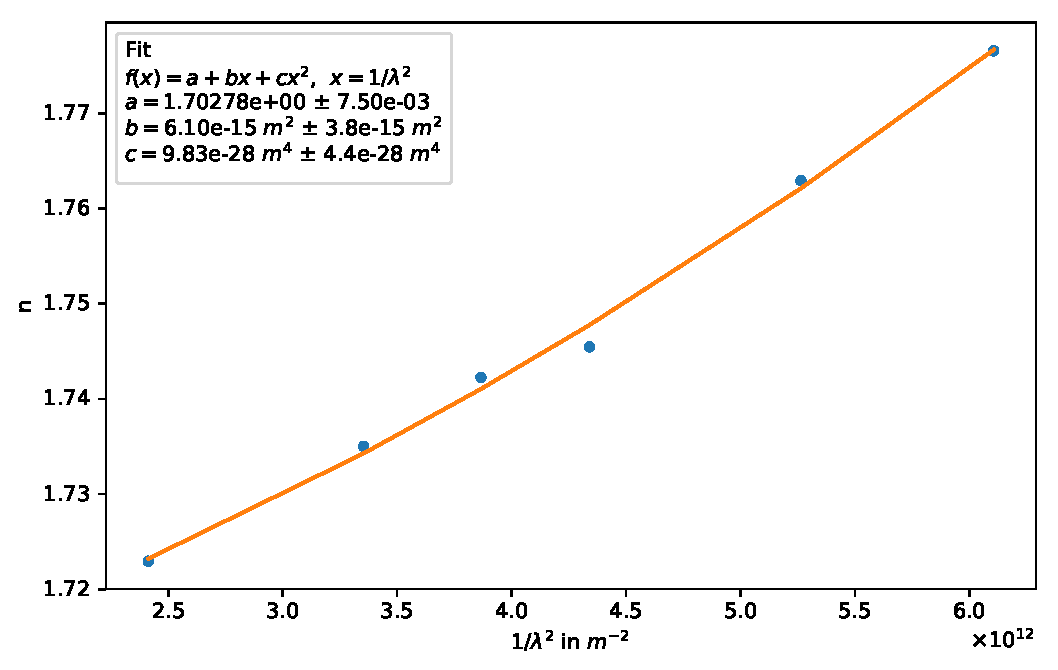
\includegraphics[width=0.7\linewidth]{Python/CdHg_Fit_Messfehler.pdf}
	\caption{Anpassung der Dispersionskurve mit der Cauchyformel}
	\label{CdHg_Fit_Messfehler}
\end{figure}
\begin{figure}[H]
	\centering
	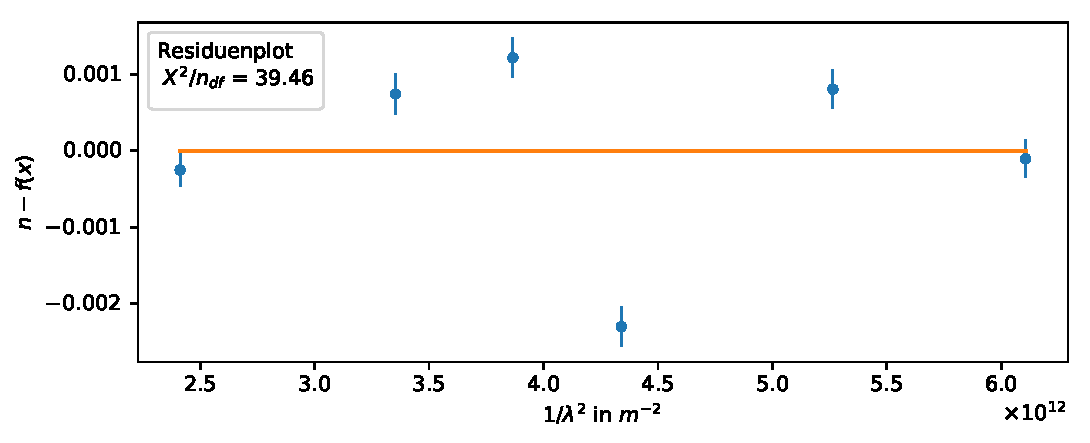
\includegraphics[width=0.7\linewidth]{Python/CdHg_Residuen_Messfehler.pdf}
	\caption{Residuenplot}
	\label{CdHg_Residuenplot_Messfehler}
\end{figure}
Die Ergebnisse der Angleichung sind in Abb.~\ref{CdHg_Fit_Messfehler} und Abb.~\ref{CdHg_Residuenplot_Messfehler} dargestellt. Im Residuenplot ist erkennbar, dass der Brechungsindex von $\lambda=479.99nm$ (hellblau) stark von der gefitteten Kurve abweicht. Dieser Wert ist vermutlich auch der Grund für den großen Wert von $\chi^2/n_{df}=39.46$. Wir stellen fest, dass die linksseitigen Winkel $\psi_1$ der hellblauen Linie zu nah an den Werten der blaugr"unen liegt und vermuten einen Messfehler. Deshalb entschließen wir uns, die Messung der hellblauen Spektrallinie nicht in die weitere Auswertung mit einzubeziehen und wiederholen die Funktionsanpassung mit den restlichen fünf Punkten(Gl.~\eqref{fitfunktion}).
\begin{figure}[H]
	\centering
	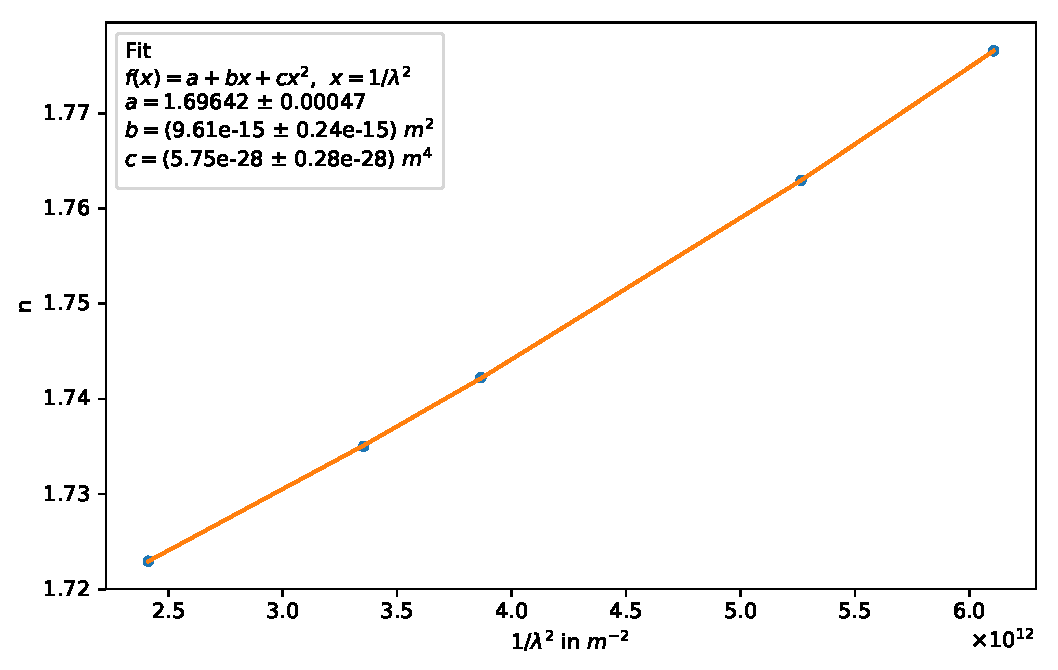
\includegraphics[width=0.7\linewidth]{Python/CdHg_Fit.pdf}
	\caption{Anpassung der Dispersionskurve mit korrigierten Werten}
	\label{CdHg_LinReg}
\end{figure}
\begin{figure}[H]
	\centering
	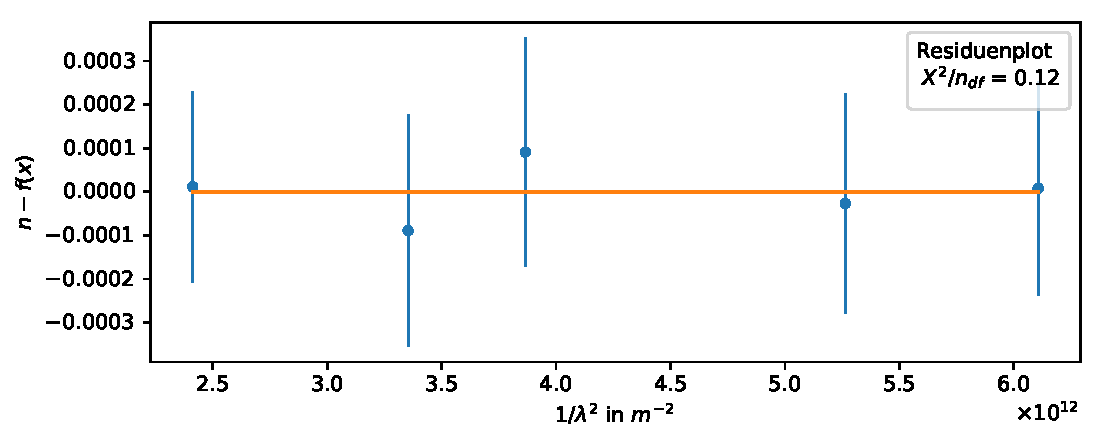
\includegraphics[width=0.7\linewidth]{Python/CdHg_Residuen.pdf}
	\caption{Residuenplot}
	\label{CdHg_Residuenplot}
\end{figure}
Die Ergebnisse sind in Abb.~\ref{CdHg_LinReg} dargestellt. Im Residuenplot (Abb.~\eqref{CdHg_Residuenplot}) ist erkennbar, dass sich die restlichen Messwerte sehr gut mit einer Parabel beschreiben lassen. Das $\chi^2/n_{df}$ ergibt 0.12, was ein Hinweis für zu groß angenommene Fehler ist. Zu groß angenommene Unsicherheiten sind nicht unplausibel, da die Rauschmessung der $\psi$ am Anfang des Versuchs durchgeführt wurde und sich das Geschick der Experimentatoren im Laufe des Versuchs verbessert haben könnte. Außerdem wurde die Rauschmessung nur für einen Experimentator durchgeführt, die Messgenauigkeit des zweiten Experimentators könnte sich von dem ersten unterscheiden.\\
Für die Parameter der quadratischen Fitfunktion erhalten wir
\begin{align}\label{Parameterwerte}
a&=1.69642\pm0.00047\\
b&=(9.61\pm0.24)10^{-15}m^2\nonumber\\
c&=(5.75\pm0.28)10^{-28}m^4\nonumber
\end{align}
Bei manchen Materialien ist bereits eine lineare Näherung $f(x)=a+bx=a+b/\lambda^2$ ausreichend, um die Dispersionskurve hinreichend genau darzustellen. Da die Abweichung $\sigma_c$ in unserer quadratischen Anpassung um eine Größenordnung kleiner ist als der Wert von $c$ selbst, können wir die quadratische Ordnung jedoch nicht weglassen und werden somit für den nächsten Teilversuch die Parameterwerte aus Gl.~\eqref{Parameterwerte} nutzen:
\begin{equation}\label{eq:fitfunction}
f(x)=1.69642+9.61\cdot10^{-15}m^2x+5.75\cdot10^{-28}m^4x^2
\end{equation}
Wir vermuten abschließend, dass es sich bei unserem Prisma um ein besonders stark brechendes Flintglas handelt. Zwar ist im Praktikumsskript kein Material mit diesem hohen Brechungsindex aufgelistet ist, allerdings gibt es verschiedene Arten von Flintglas mit Brechungsindexen im Bereich von n=1.58 bis n=1.85 (Quelle: Schott - Optisches Glas).\\

\FloatBarrier
\section{Untersuchung des Spektrums einer Zinklampe}
\subsection{Versuchsdurchführung}
Nachdem die Dispersionskurve im letzten Teilversuch bestimmt wurde, wird nun das Spektrum einer Zinklampe vermessen. Wie im vorherigen Teil werden dafür jeweils drei links- und rechtsseitige Umkehrwinkel $\psi_1$ und $\psi_2$ gemessen zu vier verschiedenen Spektrallinien. Mithilfe der Dispersionskurve können nun die Wellenlängen dieser Spektrallinien berechnet werden und mit den Literaturwerten verglichen werden.
\subsection{Auswertung}
Die links- und rechtsseitigen Umkehrwinkel der vier betrachteten Spektrallinien werden in Tabelle \ref{table:Winkel_Rohdaten_Zn} zusammengefasst. Analog zum vorherigen Teilversuch mit der Hg/Cd-Lampe wird daraus für alle Spektrallinien der Brechungsindex einschließlich Unsicherheit berechnet. Die Ergebnisse werden in Tabelle \ref{table:Zn_Rechnung} aufgelistet.\\
\begin{table}[H]
	\centering
	\begin{tabular}{|c|c|c|}
		\hline
		& Winkel $\psi_{1i}$ in Grad & Winkel $\psi_{2i}$ in Grad\\
		\hline
		Zink&$322.5+\frac{22}{60}$&$204.5+\frac{11}{60}$\\[0.1cm]
		rot&$322.5+\frac{22}{60}$&$204.5+\frac{11}{60}$\\[0.1cm]
		$\lambda=636.23nm$&$322.5+\frac{20}{60}$&$204.5+\frac{12}{60}$\\[0.1cm]
		\hline
		Zink&$325.5+\frac{12}{60}$&$201.5+\frac{16}{60}$\\[0.1cm]
		blau 1&$325.5+\frac{14}{60}$&$201.5+\frac{17}{60}$\\[0.1cm]
		$\lambda=481.05nm$&$325.5+\frac{14}{60}$&$201.5+\frac{17}{60}$\\[0.1cm]
		\hline
		Zink&$326+\frac{1}{60}$&$201.5+\frac{0}{60}$\\[0.1cm]
		blau 2&$326+\frac{1}{60}$&$201.5+\frac{0}{60}$\\[0.1cm]
		$\lambda=472.22nm$&$326+\frac{1}{60}$&$201.5+\frac{0}{60}$\\[0.1cm]
		\hline
		Zink&$326+\frac{10}{60}$&$201+\frac{21}{60}$\\[0.1cm]
		blau 3&$326+\frac{9}{60}$&$201+\frac{21}{60}$\\[0.1cm]
		$\lambda=468.01nm$&$326+\frac{9}{60}$&$201+\frac{20}{60}$\\[0.1cm]
		\hline
	\end{tabular}
	\caption{Winkel der Spektrallinien von Zn}
	\label{table:Winkel_Rohdaten_Zn}
\end{table}
\begin{table}[H]
	\centering
	\begin{tabular}{|c|c|c|c|c|c|c|}
		\hline
		&&&&&&\\
		$\lambda$ [nm] (Literaturwert)&$\overline{\psi_{1i}}\ [^{\circ}]$&$\overline{\psi_{2i}}\ [^{\circ}]$&$\delta_{min}\ [^{\circ}]$&$\sigma_{\delta_{min}}[10^{-4}\ ^{\circ}]$& $n$ & $\sigma_{n}[10^{-5}]$\\
		\hline
		$636.23$&$322.856$&$204.689$&$59.0833$&$1.4$&$1.72400$&$7.0$\\
		$481.05$&$325.722$&$201.778$&$61.9722$&$1.4$&$1.74900$&$6.7$\\
		$472.22$&$326.022$&$201.500$&$62.2611$&$1.4$&$1.75144$&$6.7$\\
		$468.01$&$326.156$&$201.344$&$62.4056$&$1.4$&$1.75266$&$6.7$\\
		\hline
	\end{tabular}
	\caption{Übersicht zur Berechnung der Zn Spektrallinien}
	\label{table:Zn_Rechnung}
\end{table}
Die aus dem ersten Versuch erhaltene Dispersionkurve $n(\lambda)=f(x)$ ist auf dem für uns relevanten Bereich streng monoton steigend bezüglich $x=\frac{1}{\lambda^2}$ und ist bei positivem $\lambda$ umkehrbar. Die Umkehrfunktion lautet:
\begin{equation}
\lambda=\lambda(n)=\sqrt{\frac{2c}{-b+\sqrt{b^2-4c(a-n)}}}
\end{equation} 
Mit dieser Formel berechnen wir die Wellenlängen der Spektrallinien zu $\lambda_{rot}=636.1nm$, $\lambda_{blau1}=481.08nm$, $\lambda_{blau2}=472.14nm$ und $\lambda_{blau3}=467.91nm$. Um den Fehler auf diese Werte abzuschätzen, berücksichtigen wir die experimentell bestimmte statistische Unsicherheit auf den Brechungsindex $n$ und berechnen ein oberes und unteres $\sigma$-Intervall für die Wellenlänge:
\begin{align}
\lambda_{+\Delta}=\lambda(n)+\sigma_{+}=\lambda(n-\sigma_n)\\
\lambda_{-\Delta}=\lambda(n)-\sigma_{-}=\lambda(n+\sigma_n)
\end{align}
Es gilt $\sigma_+\approx\sigma_-\equiv\sigma_{\lambda}$, weil sich $f(x)$ auf diesem kleinen Intervall linear nähern lässt. Die Unsicherheiten auf die Parameter $a$, $b$ und $c$ der Fitfunktion werden vernachlässigt, weil diese Unsicherheiten, dadurch dass die quadratische Angleichung mit 8 Punkten durchgeführt wurde, klein sind gegenüber der Unsicherheit auf $n$, die einem einzelnen Punkt in der Dispersionskurve entspricht. Die Unsicherheiten lauten somit für die rote Linie $\sigma_{\lambda}=0.73nm$, für die 1. blaue $\sigma_{\lambda}=0.25nm$, für die 2. blaue $\sigma_{\lambda}=0.24nm$ und für die 3. blaue $\sigma_{\lambda}=0.23nm$. Die berechneten Wellenlängen werden mit ihren Literaturwerten verglichen (Quelle:Praktikumsskript) und wir stellen fest, dass die erwarteten Wellenlängen für alle vier Spektrallinien gut mit den experimentellen Werten übereinstimmen und innerhalb der berechneten $1\sigma$-Intervallen liegen. Die Ergebnisse werden in den Abbildungen \ref{Zn_0},\ref{Zn_1},\ref{Zn_2} und \ref{Zn_3} zusammengefasst.
\begin{figure}[H]
	\centering
	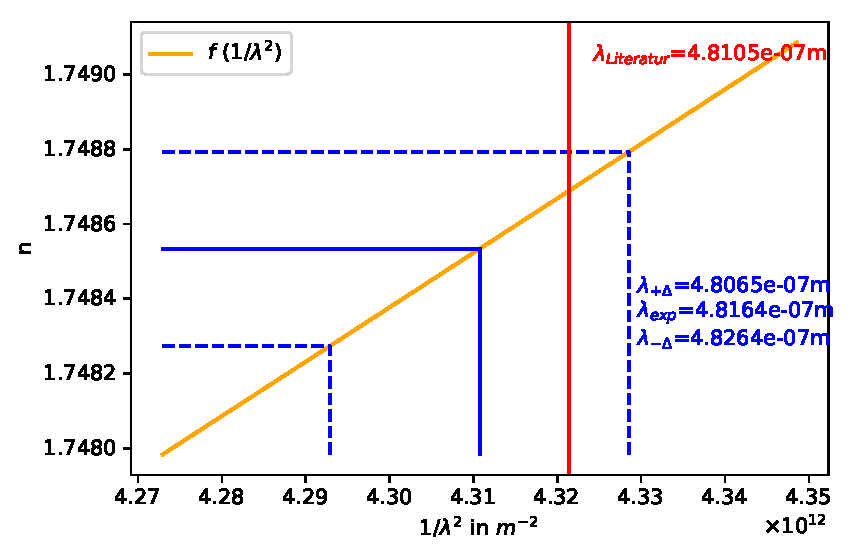
\includegraphics[width=0.7\linewidth]{Python/Zn_0.pdf}
	\caption{Wellenlängenbestimmung des Zinkspektrums: rote Linie. Vergleich mit Literaturwert.}
	\label{Zn_0}
\end{figure}

\section{Auflösungsvermögen}
\subsection{Versuchsaufbau und -durchführung}
Schließlich wird das Auflösungsvermögen des Prismas bei unterschiedlicher Ausleuchtung anhand der gelben Hg-Doppellinie bestimmt. Die Literaturwerte der dazugehörenden Wellenlängen liegen bei $\lambda_1=576.96nm$ und $\lambda_2=579.07nm$. Der Versuchsaufbau wird um eine verschiebbare Schlitzblende ergänzt, die an das vordere Ende des Kollimators befestigt wird. Die Spaltbreiten $s$ lassen sich in Schritten von 0.5mm von $s=0.5mm$ bis $s=6mm$ einstellen und bestimmen die Breite des Lichtbündels, das auf das Prisma fällt. Das Auflösungsvermögens des Prismas ist somit bestimmbar durch
\begin{equation}\label{Aufloesungsvermoegen_Prisma}
A=\Big|\frac{dn}{d\lambda}2s\frac{\sin{\frac{\epsilon}{2}}}{\cos{\frac{\delta_{min}+\epsilon}{2}}}\Big|.
\end{equation}
Die Spaltbreite wird zu kleineren Werten hin variiert und der Wert für $s$ notiert, bei der die Hg-Doppellinie gerade nicht mehr auflösbar erscheint.
\subsection{Auswertung}
Wie erwartet verschwimmen die beobachteten, gelben Hg-Doppellinien mit diskret kleiner werdendem Spaltabstand. Der Experimentator ist der subjektiven Meinung, dass sich die Linien bei einer Spaltbreite von 1.5mm noch trennen lassen, die Linien dagegen bei einer Spaltbreite von 1mm verschmelzen.\\
Das benötigte Auflösungsvermögen der Hg-Doppellinie beträgt:
\begin{equation}
A_{theo}=\frac{\lambda}{\Delta\lambda}=\frac{576.96nm}{2.11nm}=273.4
\end{equation}
Für ein Lichtbündel der Breite $s$ erwarten wir ein Auflösungsvermögen des Prismas gemäß Gl.~\ref{Aufloesungsvermoegen_Prisma}. Die Ableitung des Brechugnsindexes erhalten wir durch die in Teilversuch 1 ermittelte Ausgleichsfunktion $n(\lambda)=f(x)$. 
\begin{equation}
\frac{dn}{d\lambda}=-\frac{2b}{\lambda^3}-\frac{4c}{\lambda^5}
\end{equation}
Den minimalen Ablenkwinkel $\delta_{min}$ könnte man bei der Wellenlänge $\lambda=579.07nm$ aus Tabelle \ref{table:CdHg_Rechnung} ablesen. Wie in Abb.~\ref{CdHg_Residuenplot} erkennbar, weichen die Messergebnisse jedoch gerade bei dieser Wellenlänge relativ weit von der ermittelten Ausgleichsfunktion $f(x)$ ab (zweiter Punkt von links in Abb.~\ref{CdHg_Residuenplot}). Daher berechnen wir $\delta_{min}$ mithilfe der Fitfunktion $f(x)$ und dem Zusammenhang zwischen $n$ und $\delta_{min}$ (Gl.~\eqref{eq:n_aus_delmin}) bei $\lambda=576.96nm$:
\begin{equation}
\delta_{min}=2\arcsin\left(n(\lambda=578.96nm)\sin{\frac{\epsilon}{2}}\right)-\epsilon=\ang{56.119}.
\end{equation}
Insgesamt ergibt das Auflösungsvermögen
\begin{align}
\text{bei einer Spaltbreite von }s=1mm:A&=256.6\\
\text{bei einer Spaltbreite von }s=1.5mm:A&=384.9
\end{align}
Weil das Auflösungsvermögen sehr vom subjektiven Empfinden des Experimentators abhängig ist und nur diskrete Spaltbreiten bei dem Vesuch verwendet wurden, wird auf eine Fehlerabschätzung verzichtet. Die Einschätzung des Experimentators stimmt jedoch in diesem Fall gut mit den Erwartungen überein: Bei einer Spaltbreite von 1mm liegt das Auflösungsvermögen des Prismas $A=256.6$ unterhalb des benötigten, theoretisch berechneten Auflösungsvermögens von $A_{theo}=273.4$ und die Linien sind nicht trennbar. Bei einer Spaltbreite von 1.5mm liegt das Auflösungsvermögen des Prismas $A=384.9$ oberhalb des benötigten, theoretischen Auflösungsvermögens und die Linien sind trennbar.

\section{Fazit}
Zunächst wurde die Dispersionskurve unseres Prismamaterials anhand des Hg/Cd-Spektrums bestimmt zu
\begin{equation}
n(\lambda)=(1.69719\pm0.00043)+(9.31\pm0.21)10^{-15}m^2\frac{1}{\lambda^2}+(6.20\pm0.25)10^{-28}m^4\frac{1}{\lambda^4}
\end{equation}
Anschließend wurde das Spektrum einer Zinklampe vermessen und die experimentell bestimmten Wellenlängen mit den Literaturwerten verglichen. Die Literaturwerte liegen im $1\sigma$-Intervall der berechneten Werte.
\begin{center}
\begin{tabular}{|c|c|c|c|}
 	\hline
 	Spektrallinie & $\lambda_{exp}$&$\sigma_{\lambda}$&$\lambda_{erwartet}$\\
 	\hline
 	rot&636.1nm&0.73nm&636.23nm\\
 	blau 1&481.8nm&0.25nm&481.05nm\\
 	blau 2&472.14nm&0.24nm&472.22nm\\
 	blau 3&467.91nm&0.23nm&468.01nm\\
 	\hline
\end{tabular}
\end{center}Schließlich wurde korrekt vorausgesagt, dass das Auflösungsvermögen des Prismas bei einer Ausleuchtung der Breite 1.5mm ausreichend, aber das Auflösungsvermögen bei einer Ausleuchtung der Breite 1mm zu klein ist, um die gelbe Hg-Doppellinie zu trennen.
\end{document}